%% The "\appendix" call has already been made in the declaration
%% of the "appendices" environment (see thesis.tex).

\chapter{Glossary}

\section{Units and conventions}

In this thesis a natural system of units is used, where $\hbar = c = k_B = 1$.
In this system all the energies, masses and momenta and temperatures are given in
electron-volts (eV, keV, MeV, GeV, TeV). Energy of \unit{1}{eV} is the kinetic
energy of electron accelarated by one volt, $1$ eV = $1.6 \cdot 10^{-19}$ J.
The temperature of $1$ eV corresponds in SI via $E = k_B T$ to $11604.5$ K.
The typical length scale in the thesis is $1$ fm, so conversions between
energy and length are convenient via

\begin{equation}
  E = \frac{\hbar c}{L} \,,
\end{equation}

where $\hbar c = 0.19732$ GeV $\cdot$ fm.

The thesis adopts high-energy physics convention with metric tensor

\begin{equation}
  g^{\mu\nu} = diag(1, -1, -1, -1) \,.
\end{equation}

The terms ``low energy'', ``intermediate energy'' and ``high energy'' are frequently
used throughout the thesis. The ranges are defined only approximately, table
\ref{tab:energies_convention} summarizes the convention adopted in the text.
%\section{Collider kinematics}

\section{Abbreviations}

Abbreviations used in the thesis are collected in the following table.

\begin{table}
  \begin{tabular}{ll}
    \toprule
    BUU  &   Boltzmann-Ueling-Uhlenbeck (transport equations) \\
    CGC  &   Color Glass Condensate \cite{Gelis:2010nm,Iancu:2003xm} \\
    EoS  &   Equation of State \\
    HBT  &   Hanbury-Brown Twiss correlations \cite{Lisa:2005dd} \\
    HI   &   Heavy Ion \\
    HIC  &   Heavy Ion Collisions \\
    HRG  &   Hadron Resonance Gas \\
    QCD  &   Quantum Chromodynamics \\
    QGP  &   Quark-Gluon Plasma \\
    QMD  &   Quantum Molecular Dynamics \\
    PDF  &   Parton Distribution Functions \cite{Pumplin:2002vw,Gluck:1994uf} \\
    \midrule
    Transport codes (\ref{sec:hydro_appr}) \\
    \midrule
    AMPT  & A Multi-Phase Transport \\
    BAMPS & Boltzmann Approach to Multi-Parton Scatterings \\
    GiBUU & Gie{\ss}en BUU \\
    HSD   & Hadron-String Dynamics \\
    PHSD  & Parton-Hadron-String Dynamics \\
    RQMD  & Relativistic Quantum Molecular Dynamics \\
    SMASH & Simulating Many Strongly-interacting Hadrons \\
    UrQMD & Ultrarelativistic Quantum Molecular Dynamics \\
    \midrule
    HI centers (\ref{sec:HI_exp}) \\
    \midrule
    BNL   &  Berkley National Laboratory (Berkley, USA) \\
    BNL   &  Brookhaven National Laboratory (Brookhaven, USA) \\
    CERN  &  Center for European Nuclear Research (Geneva, Switzerland) \\
    GSI   &  Gesellschaft f\"ur Schwerionenforschung (Darmstadt, Germany) \\
    JINR  &  Joint Institute for Nuclear Research (Dubna, Russia) \\
    JPARC &  Japan Proton Accelerator Research Complex (Tsukuba, Japan) \\
    \midrule
    HI accelerators (\ref{sec:HI_exp}) \\
    \midrule
    AGS & Alternating Gradient Synchrotron \\
    HERA &  Hadron-Electron Ring Accelerator \\
    NICA &  Nuclotron-based Ion Collider Facility \\
    SIS  &  Schwerionensynchrotron \\
    SPS  &  Super Proton Synchrotron \\
    RHIC &  Relativistic Heavy Ion Collider \\
    LHC  &  Large Hadron Collider \\
    \bottomrule
  \end{tabular}
\end{table}

\chapter{Sampling two Poissonian integers $A$ and $B$ with fixed $N = A - B$}
\label{app:sampling}

In the algorithms described in chapter \ref{chap:forced_therm}  one needs to
sample ${N_1}$ and ${N_2}$ such that $w({N_1},{N_2}) \sim
\frac{\nu_1^{N_1}}{{N_1}!} \frac{\nu_2^{N_2}}{{N_2}!} \delta({N_1}-{N_2} = N)$,
$N > 0$. Let us rewrite it in terms of distribution for $N_2$:

\begin{eqnarray}
  w(N_2) = \sum_{N_1=0}^{\infty} w(N_1,N_2) \sim
           \frac{\nu_1^{N_2+N}}{(N_2+N)!} \frac{\nu_2^{N_2}}{N_2!} \\
  w(N_2) = const \frac{(\nu_1 \nu_2)^{N_2}}{N_2!(N+N_2)!}
\end{eqnarray}

Denoting $a = 2\sqrt{\nu_1 \nu_2}$ and normalizing probabilities, one obtains

\begin{equation}
  w(N_2) = \frac{a^{2N_2 + N}}{I_N(a) N_2! (N+N_2)!}
\end{equation}

This is the known Bessel distribution. The recommendations for sampling it are taken
from the paper by Yuan and Kalbfleisch \cite{Yuan2000}. Maximal probability for
the Bessel distribution is reached for

\begin{equation}
  m = \frac{1}{2} \left(\sqrt{a^2 + N^2} - N \right)
\end{equation}

It is suggested by \cite{Yuan2000} that for $m > 6$ the Bessel distribution is
very close to the Gaussian distribution, and for $m \leq 6$ probabilities can
be computed explicitly and the number can be sampled from a discrete
distribution. Moments of $Y \sim Bes(N,a)$ can be computed as

\begin{eqnarray}
  EY = \frac{1}{2} a R_N(a) \\
  EY^2 = EY \left( 1 + \frac{1}{2} a R_{N+1}(a)\right) \,,
\end{eqnarray}

Then the mean $\alpha$ and $\sigma$ of the Gaussian are

\begin{eqnarray}
  \alpha = EY \\
  \sigma = \sqrt{EY^2 - (EY)^2}
\end{eqnarray}

Here $R_N(a) = \frac{I_{N+1}(a)}{I_N(a)} = [\frac{2(N+1)}{a}, \frac{2(N+2)}{a},
\frac{2(N+3)}{a}, \cdots]$, where $[a_1,a_2,a_3,\cdots]$ denotes the continued
fraction $\frac{1}{a_1 + \frac{1}{a_2 + \cdots}}$.

An alternative method used by Becattini and Ferroni in \cite{Becattini:2004rq}
is to sample two numbers from Poissonian distributions and reject until the
difference is the required one. Devroye points out that this method requires
$\frac{e^a}{I_{\nu}(a)}$ rejections on average and is thus only acceptable for
moderate values of $a$ and $N$ \cite{Devroye2001}. In terms of our purposes, it
means that such method works well only for small enough chemical potentials.
For completeness let us add that in response to the approximate sampling method by
Yuan and Kalbfleisch, Devroye has suggested an exact method \cite{Devroye2001}.
However, for the purposes of chapter \ref{chap:forced_therm} the approximate method is
sufficient, as Fig. \ref{Fig:BFefix_sampling} demonstrates.

\chapter{Hadrons and the $\SUgroup{3}$ group} \label{sec:SU3}

%http://www.hep.phy.cam.ac.uk/~thomson/lectures/partIIIparticles/Handout7_2009.pdf
%http://www.hep.phy.cam.ac.uk/~thomson/lectures/partIIIparticles/Handout8_2009.pdf

Hadrons are the degrees of freedom implemented in transport models UrQMD and
SMASH used throughout this thesis. In fact, hadrons are one of the main objects
of study of the thesis. Nevertheless, two important questions about hadrons
were omitted in the main part: ''why only certain combinations of quarks and
antiquarks occur as hadrons?'' and ''how are hadrons classified?'' Both of them
are answered with the help of $\SUgroup{3}$ group. By definition $\SUgroup{3}$
group is a group of $3 \times 3$ matrices $\U$ such that $\U\U^{\dag} =
\mathbb{1}$ and $\mathrm{det} \U = 1$. In the following its role in
hadron classification and in explaining color confinement (see section
\ref{sec:confinement}) is acknowledged.

Hadrons and quarks are microscopic objects, so their properties are defined by
the quantum wavefunction $\ket{\Psi}$ - a complex function of spatial
coordinate, spin and other variables of particle internal state. The squared
module of wavefunction $\modsq{\Psi}$ is a probability to find particle at a
given coordinate in a given state. Finding the wavefunction of the quantum
system is enough to predict its properties.

For a single quark wavefunction is a product of color, flavor, spin and spatial
parts:

\begin{equation}
  \ket{\Psi} = \ket{\Psi_{\mathrm{color}}} \ket{\Psi_{\mathrm{flavor}}}
               \ket{\Psi_{\mathrm{spin}}}  \ket{\Psi(x)}
\end{equation}

Let us concentrate on the color part, which can be represented as
a complex vector with 3 components. During propagation of the free quark color
is conserved. According to Noether theorem, every conservation law corresponds
to a symmetry, which in this case is invariance of interactions under
multiplication of $\ket{\Psi_{\mathrm{color}}}$ by matrices from $\SUgroup{3}$
group, in other words invariance under color rotations.

In mathematical terms $\SUgroup{3}$ is a Lie group and it is fully defined by
its Lie algebra of infinitesimal color rotations: for every matrix $\U$ from
$\SUgroup{3}$

\begin{equation}
  \U = \expOf{\sum_{k = 1}^8 i \alpha_k \lambda_k/2} ,
\end{equation}

where $\alpha_k$ are arbitrary real numbers and $\lambda_k/2$ matrices are
called generators, which for $\SUgroup{3}$ are known as Gell-Mann matrices.
Explicitly expressed, $\lambda_k$ are

\begin{subequations} \label{eq:gell_mann}

  \begin{equation} \label{eq:lambda1-3}
  \begin{array}{ccc}
    \lambda_1 = \left(
      \begin{array}{ccc}
            0 & 1 & 0 \\
            1 & 0 & 0 \\
            0 & 0 & 0
      \end{array} \right)
    &
    \lambda_2 = \left(
      \begin{array}{ccc}
            0 & -i & 0 \\
            i &  0 & 0 \\
            0 &  0 & 0
      \end{array} \right)
    &
    \lambda_3 = \left(
      \begin{array}{ccc}
             1 &  0 & 0 \\
             0 & -1 & 0 \\
             0 &  0 & 0
      \end{array} \right)
  \end{array}
  \end{equation}


  \begin{equation} \label{lamdba4-6}
  \begin{array}{ccc}
    \lambda_4 = \left(
    \begin{array}{ccc}
           0 & 0 & 1 \\
           0 & 0 & 0 \\
           1 & 0 & 0
    \end{array} \right)
    &
    \lambda_5 = \left(
    \begin{array}{ccc}
           0 & 0 & i \\
           0 & 0 & 0 \\
          -i & 0 & 0
    \end{array} \right)
    &
    \lambda_6 = \left(
    \begin{array}{ccc}
           0 & 0 & 0 \\
           0 & 0 & 1 \\
           0 & 1 & 0
    \end{array} \right)
  \end{array}
  \end{equation}


  \begin{equation} \label{lamdba7-8}
  \begin{array}{cc}
    \lambda_7 = \left(
    \begin{array}{ccc}
           0 & 0 & 0 \\
           0 & 0 & -i \\
           0 & i & 0
    \end{array} \right)
    &
    \lambda_8 = \frac{1}{\sqrt{3}} \left(
    \begin{array}{ccc}
           1 & 0 &  0 \\
           0 & 1 &  0 \\
           0 & 0 & -2
    \end{array} \right)
  \end{array}
  \end{equation}

\end{subequations}

Choosing basis vectors in color space as

\begin{equation}
  \begin{array}{ccc}
    r = \left( \begin{array}{c} 1 \\ 0 \\ 0 \end{array} \right) &
    g = \left( \begin{array}{c} 0 \\ 1 \\ 0 \end{array} \right) &
    b = \left( \begin{array}{c} 0 \\ 0 \\ 1 \end{array} \right)
  \end{array}
\end{equation}

one can introduce ladder operators from non-diagonal Gell-Mann matrices and
color isospin projection $I_3^c$ and color hypercharge $Y_c$ operators from
diagonal matrices:

\begin{equation} \label{eq:SU3_ladder_operators}
  \begin{array}{c}
    T^{\pm} = \frac{1}{2} \left(\lambda_1 \pm i\lambda_2 \right) \\
    V^{\pm} = \frac{1}{2} \left(\lambda_4 \pm i\lambda_5 \right) \\
    \U^{\pm} = \frac{1}{2} \left(\lambda_6 \pm i\lambda_7 \right) \\
    I_3^c = \frac{1}{2} \lambda_3 \\
    Y_c = \frac{1}{\sqrt{3}} \lambda_8
  \end{array}
\end{equation}

\begin{figure}
  \centering
  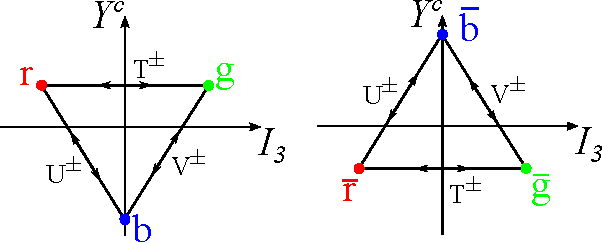
\includegraphics[width = 0.8\textwidth]{illustrations/intro_illustrations/SU3_ladder_operators.pdf}
  \caption{Ladder operators of $\SUgroup{3}$ group in space of quark
           colors.}
  \label{fig:q_color_ladder_operators}
\end{figure}

These operations turn quark and antiquark colors into each other, as
illustrated in Fig.  \ref{fig:q_color_ladder_operators}. It is postulated
that existing bound states are color singlets, meaning that acting with
matrices \ref{eq:SU3_ladder_operators} on every single quark and antiquark
turns the whole state into itself. It can be shown that this requirement
defines color parts of meson and baryon wavefunctions uniquely:

\begin{align}
  \ket{\Psi_c^{q\bar{q}}} &=& \frac{1}{\sqrt{3}} \parenths{r\bar{r} + g\bar{g} + b\bar{b}} \\
  \ket{\Psi_c^{qqq}} &=& \frac{1}{\sqrt{6}} \parenths{rgb - rbg + gbr - grb + brg - bgr}
\end{align}

Exactly the same mathematics is used for hadron classification, but now
$\SUgroup{3}$ is acting in flavor space of the lightest quarks: $u$, $d$ and
$s$. Note that $\SUgroup{3}$ color symmetry is exact, but $\SUgroup{3}$ flavor
symmetry is only approximate, because the masses of light quarks are not
identical.

Hadrons should be colorless, but they should not necessarily be flavorless. In
the other words, all the flavor representations are allowed. It can be proven
that combinations of quarks split into irreducible representations of $\SUgroup{3}$
in flavor space in the following way:

\begin{align}
  3 \bigotimes \bar{3} = 1 \bigoplus 8 \\
  3 \bigotimes 3 \bigotimes 3 = 10 \bigoplus 8 \bigoplus 8 \bigoplus 1
\end{align}

This means that there are 8 mesons (octet) that turn one into another under
$\SUgroup{3}$ flavor transformations and one meson that always turns into
itself. As for baryons - 10 baryons (decuplet) transforming into each other and
two physically equivalent octets.  The singlet absent in nature, because
strictly speaking one has to consider flavor and spin transformations together
and in the representation of $\SUgroup{3} \times \SUgroup{2}$ (the
$\SUgroup{2}$ group is here for spin transformations) flavor singlet is absent.

This explains classification of mesons into octet and singlet and baryons into
decuplet and octet as shown in Figure \ref{fig:mes_bar}, which presents the
lightest mesons and baryons consisting of $u$, $d$, $s$ quarks and their
antiquarks. Supplementing this picture by vector mesons, antibaryons and
a tower of excitations and adding those for heavier quarks one gets a zoo of
hadrons that observed in experiment. Few hadrons are discovered that may fall
out of this classification scheme. They are supposed to be tetraquarks
or 6-quark molecules.

\begin{figure}
  \centering
  \subfloat[][Mesons]{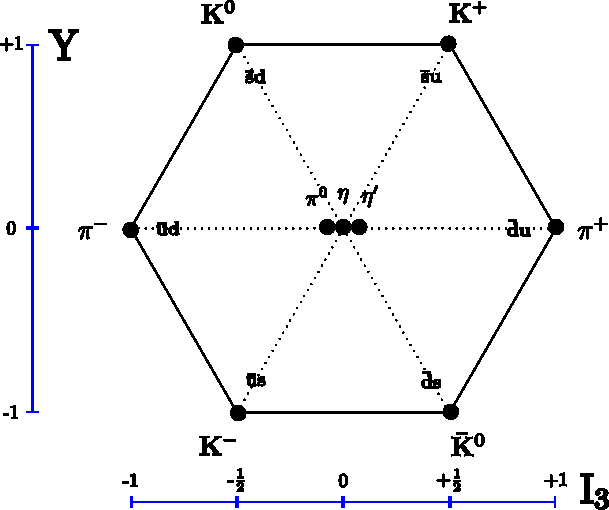
\includegraphics[height=6.5cm]{illustrations/intro_illustrations/mesons.pdf}} \hfill
  \subfloat[][Baryon octet]{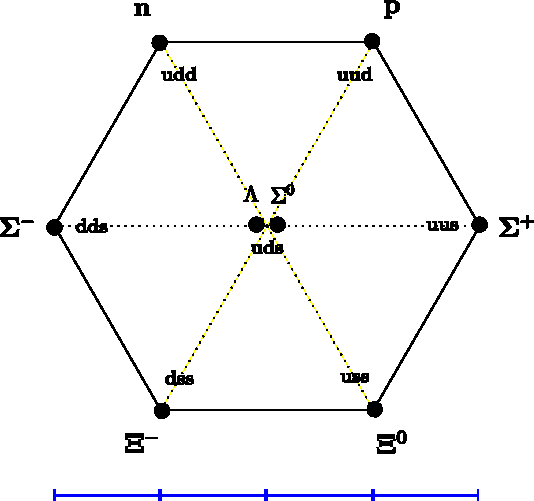
\includegraphics[height=6.5cm]{illustrations/intro_illustrations/baryon_octet.pdf}} \\
  \subfloat[][Baryon decuplet]{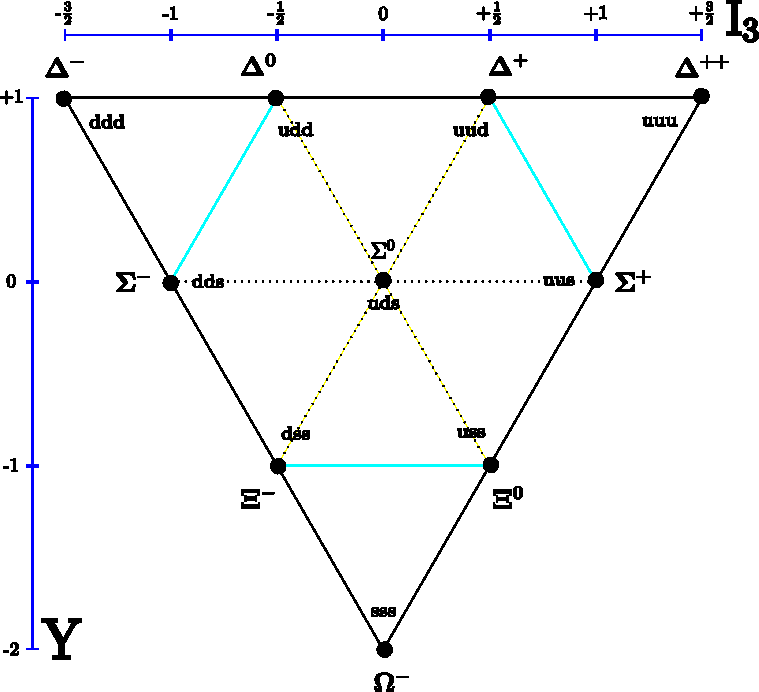
\includegraphics[height=6.5cm]{illustrations/intro_illustrations/baryon_decuplet.pdf}}
  \caption{Classification of hadrons, consisting of light quarks, in the lowest
           energy state. The picture is taken from lectures in QCD by F. Jegerlehner.}
  \label{fig:mes_bar}
\end{figure}